\documentclass{beamer}

\usefonttheme{serif}
\beamertemplatenavigationsymbolsempty
\setbeamertemplate{footline}[frame number]
\usecolortheme[named=violet]{structure}

\usepackage{geometry}
\usepackage{amssymb, amsmath, amsthm}
\usepackage{enumitem}
\usepackage{pgf,tikz}
\usepackage{listings}
\usepackage{algpseudocode}
\usepackage{svg}
\usepackage[dvipsnames]{xcolor}

\lstset{
    commentstyle=\color{SeaGreen},
    keywordstyle=\color{magenta},
    numberstyle=\tiny\color{Gray},
    stringstyle=\color{codepurple},
    basicstyle=\ttfamily\footnotesize,
    breaklines=true,                 
    captionpos=b,                    
    keepspaces=true,                 
    numbers=left,                    
    numbersep=5pt,                  
    showspaces=false,                
    showstringspaces=false,
    showtabs=false,                  
    tabsize=4,
}
\lstloadlanguages{C}

\renewcommand{\algorithmicrequire}{\textbf{Input:}}
\renewcommand{\algorithmicensure}{\textbf{Output:}}

\newcommand{\Q}{\mathbb{Q}}
\newcommand{\Z}{\mathbb{Z}}
\newcommand{\N}{\mathbb{N}}
\newcommand{\angles}[1]{\langle #1 \rangle}
\newcommand{\dd}{\mathop{}\!d}
\newcommand{\its}[1]{\textcolor{violet}{\emph{#1}}}

\DeclareMathOperator{\rev}{\text{rev}}

\newtheorem{proposition}{Proposition}

\setbeamertemplate{theorems}[normal font]

\title{COSC3500 Project}
\subtitle{Milestone 1 (serial)}
\author{Mitchell Holt}
\date{September 2024}

\begin{document}

\titlegraphic{
\includegraphics[width=.37\textwidth]{thinker.jpg}}

\begin{frame}
    \maketitle
\end{frame}

\begin{frame}
    \frametitle{The Problem}

    Let $F$ be a field and let $a,b \in F[x]$ with
    \begin{equation}
        a = \sum_{k = 0}^m a_k x^k, \qquad b = \sum_{k = 0}^n b_k x^k
    \end{equation}\pause \vfill

    Then
    \begin{equation}
        ab = \sum_{k = 0}^{m + n} c_k x^k,
            \qquad \text{where } c_k = \sum_{i = 0}^k a_i b_{k - i}
    \end{equation}
    

    \pause \vfill

    \its{Bad news:} $(N + 1)(N + 2)/2$ multiplications (where $N = \deg ab$).
\end{frame}

\begin{frame}
    \frametitle{Fast Interpolation}
    
    Let $\omega$ be a primitive $n$th root of unity (introduces symmetry) and
    $a,b \in F[x]$. \pause \vfill

    \its{Algorithm idea:}
    \begin{enumerate}[label=\arabic*.]
        \item Fast multipoint evaluation of $a$ and $b$, yielding:
            \begin{gather*}
                A = \begin{bmatrix}
                    a(1) & a(\omega) & \cdots & a(\omega^{n - 1})
                \end{bmatrix} \\
                B = \begin{bmatrix}
                    b(1) & b(\omega) & \cdots & b(\omega^{n - 1})
                \end{bmatrix}
            \end{gather*}
            \pause
        \item Compute the multipoint evaluation of the product, yielding:
            $$
                C = \begin{bmatrix}
                    A_0B_0 & A_1B_1 & \cdots & A_{n - 1}B_{n - 1}
                \end{bmatrix}
            $$
            \pause
        \item \its{Interpolate} $ab$ from $ab(\omega^i) = C_i$ ($i = 0, \dots,
            n - 1$).
    \end{enumerate}
\end{frame}

\begin{frame}
    \frametitle{Fast Multipoint Evaluation}

    $\texttt{FFT1}(n,\ \omega,\ V)$
    \begin{algorithmic}
        \Require $n = 2^k$, a primitive $n$th root of unity $\omega$, and the
        coefficient vector $V = \begin{bmatrix} a_0 & a_1 & \cdots & a_{n - 1}
        \end{bmatrix}$ of $f \in F[x]$
        \Ensure $\begin{bmatrix} f(1) & f(\omega) & \cdots & f(\omega^{n - 1})
        \end{bmatrix}$
        \pause \vfill

        \If{$n=1$} \State \Return $V$ \EndIf
        \pause \vfill

        \State $A \gets \texttt{FFT1}(n/2,\ \omega^2,\
        \begin{bmatrix} a_0 & a_2 & \cdots & a_{n - 2} \end{bmatrix})$
        \State $B \gets \texttt{FFT1}(n/2,\ \omega^2,\
        \begin{bmatrix} a_1 & a_3 & \cdots & a_{n - 1} \end{bmatrix})$
        \pause \vfill

        \For{$i=0,1,\dots,n/2 - 1$}
            \State $C_i \gets A_i + \omega^iB_i$
            \State $C_{n/2 + i} \gets A_i - \omega^iB_i$
        \EndFor
        \pause \vfill

        \State \Return $C$
    \end{algorithmic}

    \pause \vfill

    \its{Good news:} $O(n\log n)$
\end{frame}

\begin{frame}
    \frametitle{Fast Interpolation}

    $\texttt{FFT2}(n,\ \omega,\ A)$
    \begin{algorithmic}
        \Require $n = 2^k$, a primitive $n$th root of unity $\omega$, and a
        multipoint evaluation vector $A = \begin{bmatrix} f(1) & f(\omega) &
        \cdots & f(\omega^{n - 1}) \end{bmatrix}$ of $f \in F[x]$
        \Ensure The coefficient vector $V = \begin{bmatrix} a_0 & a_1 & \cdots
        & a_{n - 1} \end{bmatrix}$ of $f$.
        \pause \vfill

        \If{$n=1$} \State \Return $V$ \EndIf
        \pause \vfill

        \For{$i=0,1,\dots,n/2 - 1$}
            \State $B_i \gets A_i + A_{n/2 + i}$
            \State $C_i \gets \omega^{-i}(A_i - A_{n/2 + i})$
        \EndFor
        \pause \vfill

        \State $B \gets \texttt{FFT2}(n/2,\ \omega^2,\ B)$
        \State $C \gets \texttt{FFT2}(n/2,\ \omega^2,\ C)$
        \pause \vfill

        \State \Return $\begin{bmatrix} B_0/n & C_0/n & B_1/n & C_1/n & \cdots
        & B_{n - 1}/n & C_{n - 1}/n \end{bmatrix}$
    \end{algorithmic}

    \pause \vfill

    \its{Good news:} $O(n\log n)$
\end{frame}

\begin{frame}
    \frametitle{In-place FFT Multiplication}

    Code is adapted from Michael Monagan \cite{monagan}:

    \begin{figure}[b]
        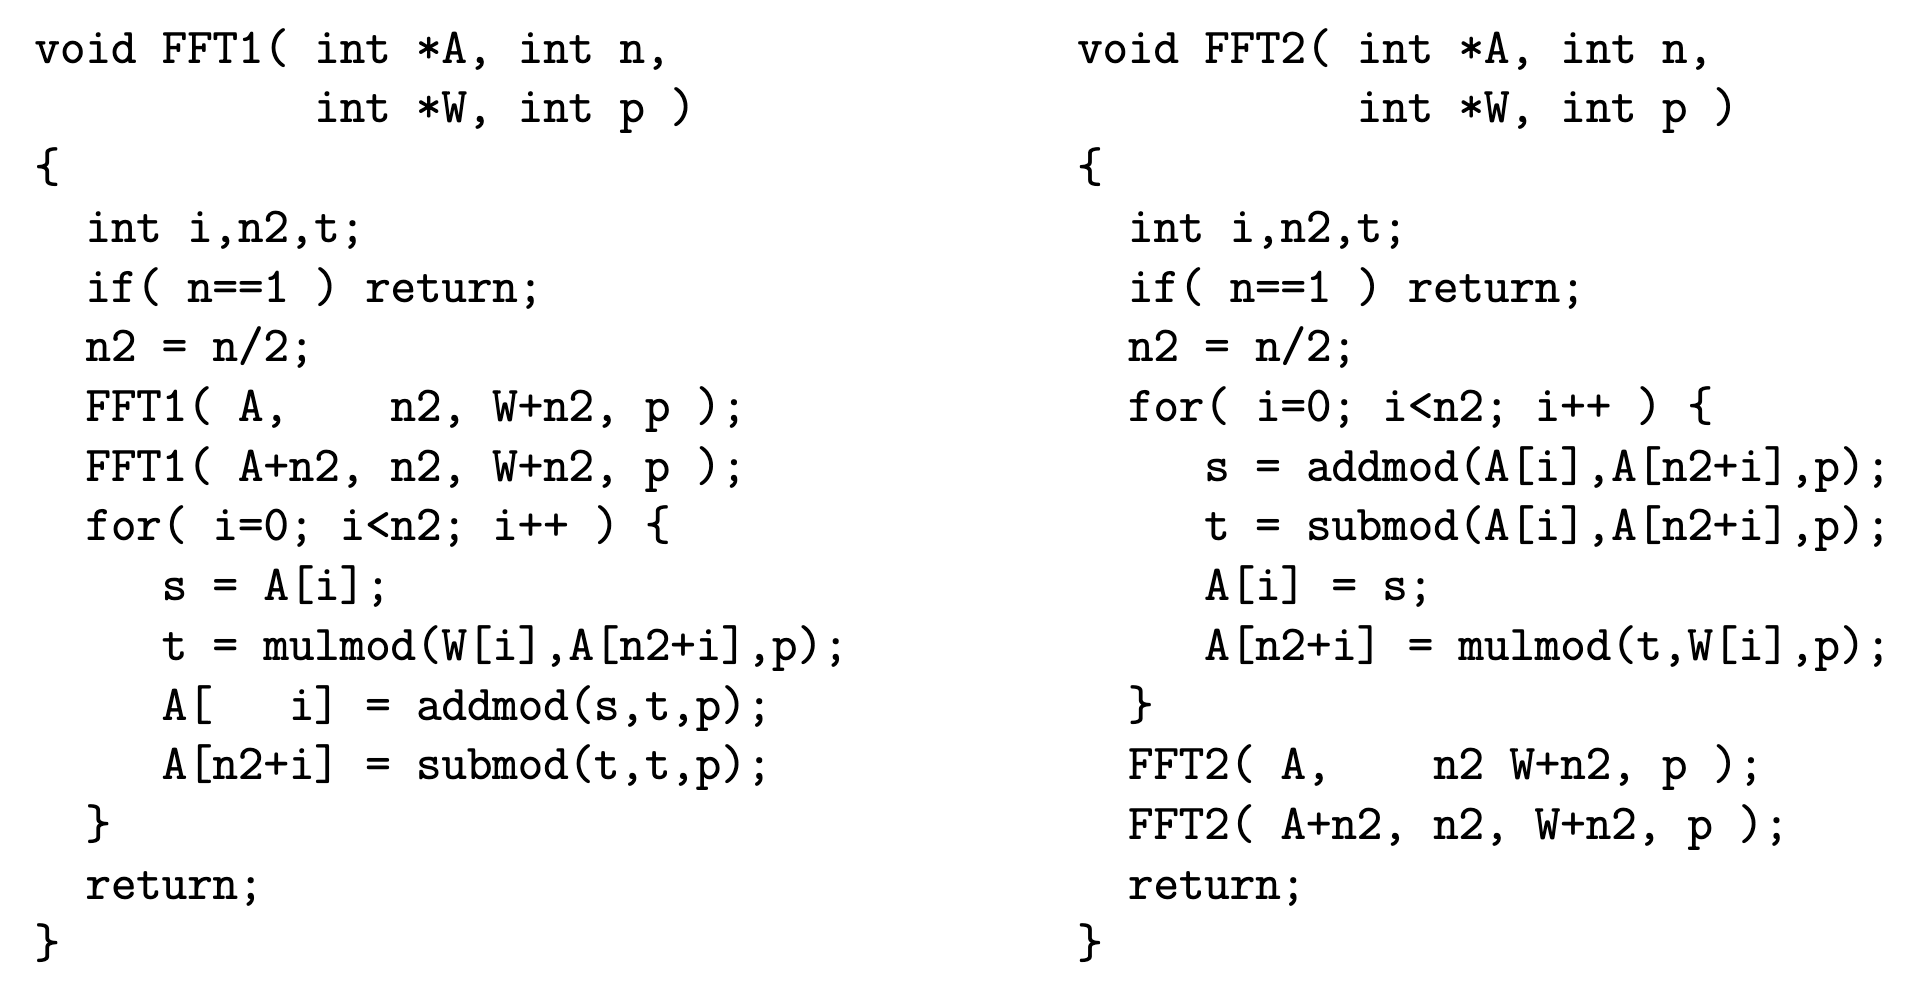
\includegraphics[width=\textwidth]{monagan.png}
    \end{figure}
\end{frame}

\begin{frame}
    \frametitle{Initial Implementation}

    \begin{enumerate}[label=(\roman*)]
        \item Working over the field $\mathbb{Z}/(2^{16} + 1)$. \pause
            \smallbreak
        \item Generate a random (and valid) $\omega$ for each polynomial
            multiplication (to simulate a real-world use case). \pause
            \smallbreak
        \item The coefficients of the polynomials \emph{cannot} make a
            difference. Generate random polynomials so the compiler doesn't
            optimise everything away. \pause \smallbreak
        \item Time the generation of $\omega$ and the polynomial multiplication.
            \pause \smallbreak
        \item Verify results with a Maple script.
    \end{enumerate}
\end{frame}

\begin{frame}
    \frametitle{Results}

    Ran 1000 examples for each degree. Report average timings

    \begin{figure}
        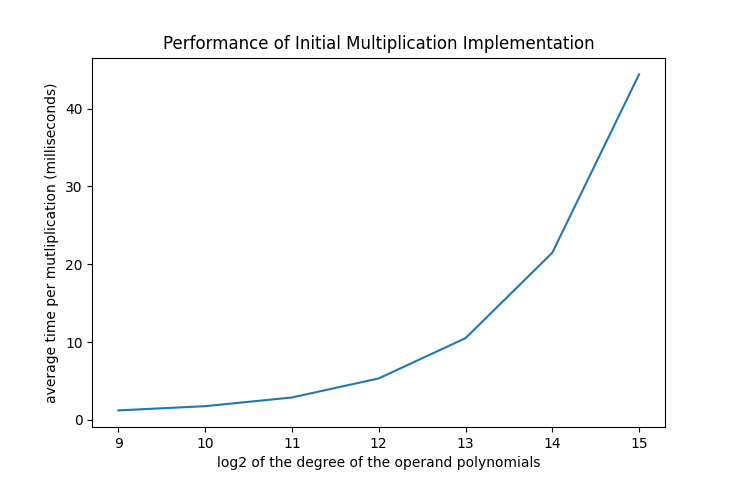
\includegraphics[width=\textwidth]{initial.png}
    \end{figure}
\end{frame}

\begin{frame}
    \frametitle{Fast Field Inverse}

    \begin{enumerate}[label=(\roman*)]
        \item Compute exactly two field inverses per polynomial multiplication
            \pause \smallbreak
        \item Profiler shows 37\% of runtime spent in \texttt{invmod}:
            \lstinputlisting[language=C]{init_invmod}
            \pause \smallbreak
        \item \texttt{powmod} is \its{linear} in $n$. \pause We can use repeated
            squaring to make it \its{logarithmic}.
    \end{enumerate}
\end{frame}

\begin{frame}
    \frametitle{Results}
    
    Ran 1000 examples for each degree. Report average timings.

    \begin{figure}
        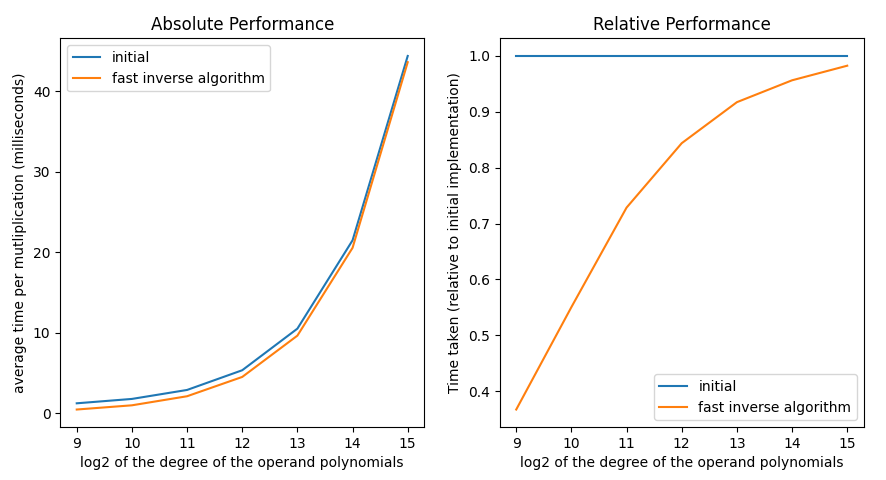
\includegraphics[width=\textwidth]{fastinv.png}
    \end{figure}
\end{frame}

\begin{frame}
    \frametitle{Fast Field Multiplication}

    \begin{enumerate}[label=(\roman*)]
        \item Initial implementation uses modulo operator:
            \lstinputlisting[language=C]{mulmod} \pause \smallbreak
        \item We can compute the product without mod:
            \lstinputlisting[language=C]{mulmod_slow} \pause \smallbreak
        \item Bit hack method is slightly slower (!)
    \end{enumerate}
\end{frame}

\begin{frame}
    \frametitle{Cache Locality for Pointwise Multiplication}

    \begin{enumerate}[label=(\roman*)]
        \item Initial code:
            \lstinputlisting[language=C]{no_blocking}
            \pause \smallbreak
        \item Optimised loop (using stack array \texttt{bbuf}) \pause:
            \lstinputlisting[language=C]{blocking}
            \pause \smallbreak
        \item There are $64\text{bytes}/8\text{bytes} = 16$ ints in a cache
            line, but \texttt{BLOCK\_INTS=4} is the sweet spot for perfomance
    \end{enumerate}
\end{frame}

\begin{frame}
    \frametitle{Results}
    
    Ran 1000 examples for each degree. Report average timings.

    \begin{figure}
        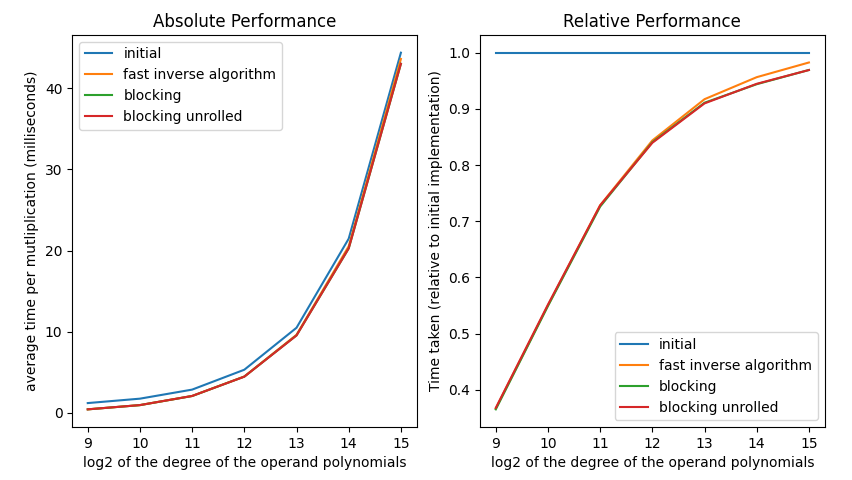
\includegraphics[width=\textwidth]{fastmult.png}
    \end{figure}
\end{frame}

\begin{frame}
    \frametitle{Precomputing $\omega$ Powers Array}

    Need to compute (following \cite{monagan}):
    \begin{equation*}
        W = \big[
            \underbrace{\omega^0, \omega^1, \cdots, \omega^{n/2 - 1}}_{n/2 \text{ elems}},
            \underbrace{\omega^0, \omega^2, \cdots, \omega^{n/2 - 2}}_{n/4},
            \underbrace{\cdots}_{n/8,\dots,2},
            \underbrace{\omega^0}_{1},
            0
        \big]
    \end{equation*}
    
    \pause \vfill

    \begin{enumerate}[label=(\roman*)]
        \item Initial implementation does $n/2$ field multiplications,
            but has poor cache locality for $W$. \pause \smallbreak
        \item Tried an implementation that moves linearly along $W$ and does $n$ 
            field multiplications. \pause This is slower.
    \end{enumerate}
\end{frame}

\begin{frame}
    \frametitle{Loop Unrolling and Cache Locality in FFT}

    \begin{enumerate}[label=(\roman*)]
        \item Initial loop code:
            \lstinputlisting[language=C]{fft_loop_old}
            \pause \smallbreak
        \item Optimised loop (using stack arrays \texttt{bbuf} and
            \texttt{wbuf}): \pause
            \lstinputlisting[language=C]{fft_loop_new}
    \end{enumerate}
\end{frame}

\begin{frame}
    \frametitle{Results}
    
    Ran 1000 examples for each degree. Report average timings.

    \begin{figure}
        \includegraphics[width=\textwidth]{fft.png}
    \end{figure}
\end{frame}

\begin{frame}
    \frametitle{References}

    \bibliographystyle{alpha}
    \bibliography{bibliography}
\end{frame}

\end{document}
